\chapter{Trabajo relacionado}

\section{Inteligencia artificial}

La inteligencia artificial (IA), en el contexto de las ciencias de la computación, es una disciplina y un conjunto de capacidades cognoscitivas e intelectuales expresadas por sistemas informáticos o combinaciones de algoritmos cuyo propósito es la creación de máquinas que imiten la inteligencia humana para realizar tareas, y que pueden mejorar conforme recopilen información\cite{espanola2014diccionario}. Se hizo presente poco después de la Segunda Guerra Mundial con el desarrollo de la "prueba de Turing", mientras que la expresión "inteligencia artificial" fue acuñada en 1956 por el informático John McCarthy en la Conferencia de Dartmouth.

En la actualidad, la inteligencia artificial abarca una gran variedad de subcampos. Éstos van desde áreas de propósito general, aprendizaje y percepción, a otras más específicas como el reconocimiento de voz, el juego de ajedrez, la demostración de teoremas matemáticos y el diagnóstico de enfermedades. La inteligencia artificial sintetiza y automatiza tareas que en principio son intelectuales y, por lo tanto, es potencialmente relevante para cualquier ámbito de actividades intelectuales humanas. En este sentido, es un campo genuinamente universal.

En cuanto a su clasificación, tradicionalmente se divide a la inteligencia artificial en inteligencia artificial débil, la cual es la única que existe en la actualidad y que se ocupa de realizar tareas específicas, e inteligencia artificial fuerte, que sería una IA que excediese las capacidades humanas. Algunos expertos creen que si alguna vez se alcanza este nivel, se podría dar lugar a la aparición de una singularidad tecnológica, es decir, una entidad tecnológica superior que se mejoraría a sí misma constantemente, volviéndose incontrolable para los humanos, dando pie a teorías como el basilisco de Roko.\cite{basilico}

Stuart J. Russell y Peter Norvig diferencian varios tipos de inteligencia artificial:

\begin{itemize}
\item Sistemas que piensan como humanos
\item Sistemas que actúan como humanos  
\item Sistemas que piensan racionalmente
\item Sistemas que actúan racionalmente
\end{itemize}

\subsection{Redes neuronales artificiales}

Las redes neuronales artificiales (RNA) son un paradigma de aprendizaje y procesamiento automático inspirado en la forma en que funciona el sistema nervioso de los animales. Se trata de un sistema de interconexión de neuronas en una red que colabora para producir un estímulo de salida. En inteligencia artificial es frecuente referirse a ellas como redes neuronales o redes neuronales artificiales para distinguirlas claramente de las redes neuronales biológicas.

La misma está constituida por neuronas interconectadas y arregladas en tres capas (esto último puede variar). Los datos ingresan por medio de la "capa de entrada", pasan a través de la "capa oculta" y salen por la "capa de salida". Cabe mencionar que la capa oculta puede estar constituida por varias capas. Antes de comenzar el estudio sobre las redes neuronales, se debe aprender algo sobre las neuronas y de cómo ellas son utilizadas por una red neuronal.

\begin{figure}[h]
    \centering
    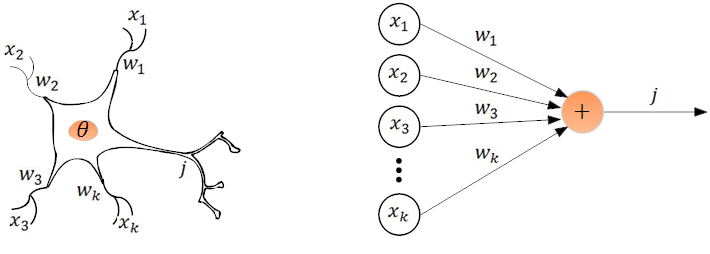
\includegraphics[width=.8\textwidth]{images/Figura-7-Neurona-biologica-versus-artificial-Una-neurona-artificial-es-una-unidad-de.png}
    \caption{Comparación red neuronal biológica(izquierda) y una artificial(derecha)}
    \label{fig:neurona_biologica_artificial}
\end{figure}

Se pueden observar las similitudes entre ambas (tienen entradas, utilizan pesos y generan salidas).

Mientras una neurona es muy pequeña en sí misma, cuando se combinan cientos, miles o millones de ellas pueden resolver problemas muy complejos. El objetivo de la red neuronal es resolver los problemas de la misma manera que el cerebro humano, aunque las redes neuronales son más abstractas. Las redes neuronales actuales suelen contener desde unos miles a unos pocos millones de unidades neuronales.

La inteligencia artificial deriva en una serie de modelos o ramas que se pueden emplear en diferentes ámbitos de la vida de las personas, así como en el mundo profesional para automatizar procesos que, realizados de manera tradicional, pueden resultar poco productivos, ineficientes, lentos o costosos.

Cada subcampo de la inteligencia artificial se encuentra en constante cambio y actualización. Por tanto, se prevé que aparezcan muchos más y que con el tiempo otros vayan quedando "obsoletos", dejen de utilizarse, o saquen versiones mejoradas sin eliminar ese tipo de IA (como ocurre, por ejemplo, con el Deep Learning y el Machine Learning).

Se aborda dos conceptos englobados dentro de la inteligencia artificial que conforman las técnicas utilizadas en este proyecto. Esas dos técnicas son las llamadas redes neuronales artificiales y los algoritmos genéticos.

\subsection{Algoritmos genéticos}

Los algoritmos genéticos (GA, del inglés genetic algorithms) son algoritmos de búsqueda basados en los mecanismos de selección y genética natural. Los algoritmos genéticos combinan la supervivencia del mejor adaptado entre estructuras de secuencias con un intercambio de información estructurado, aunque aleatorizado, para constituir así un algoritmo de búsqueda que tenga algo de las genialidades de las búsquedas humanas.

En cada iteración, los algoritmos genéticos mantienen una población de estructuras que son los candidatos de soluciones que compiten según un criterio de bondad para resolver el problema. Los operadores inspirados en la genética natural como son la selección, el cruce y la mutación actúan sobre dichas estructuras formando nuevos candidatos de solución.

La manera de estructurar un algoritmo genético es la siguiente:
\begin{enumerate}
\item[t = 0:] Inicializar una población P(t)
\item[t = 1:] Evaluar P(t)
\item[t = 2:] Mientras no se cumpla la condición de parada hacer:
\begin{itemize}
\item Seleccionar P(t)
\item Aplicar operadores genéticos a P(t) para crear P(t+1) 
\item Evaluar P(t+1)
\item t = t+1
\end{itemize}
\end{enumerate}

El algoritmo genético trabaja con una codificación de parámetros, no con los parámetros en sí mismos. Explora simultáneamente muchos puntos del espacio de búsqueda, no sólo uno. Utiliza información de la función objetivo, no derivadas u otros conocimientos auxiliares. Emplea transiciones probabilísticas, no reglas determinísticas.

Los algoritmos genéticos difieren de los métodos de optimización más tradicionales en cuatro aspectos fundamentales:
\begin{itemize}
\item Trabajan con una codificación del conjunto de parámetros, no con los parámetros en sí mismos.
\item Realizan la búsqueda a partir de una población de puntos, no de un único punto.
\item Utilizan información de la función objetivo, no derivadas ni ningún otro conocimiento auxiliar.
\item Utilizan reglas de transición probabilísticas, no determinísticas.
\end{itemize}

\begin{figure}[h]
    \centering
    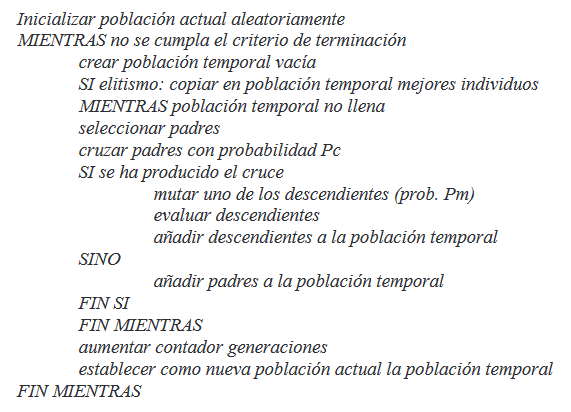
\includegraphics[width=.8\textwidth]{images/pseudocodigo.png}
    \caption{Funcionamiento algoritmo genético}
    \label{fig:pseudocodigo_algoritmo_genetico}
\end{figure}

El funcionamiento genérico de un algoritmo genético puede apreciarse en el pseudocódigo, reflejado en la figura \ref{fig:pseudocodigo_algoritmo_genetico}acionado}


\section{Inteligencia artificial\begin{figure}[h]
    \cen    \centering
    \includegraphics[width=.8\textwidth]{images/Figura-7-Neurona-biologica-versus-artificial-Una-neu\begin{figure}[h]
    \centering
    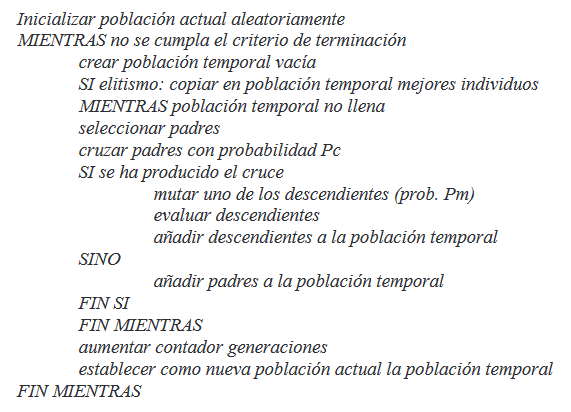
\includegraphics[width=.8\textwidth]{images/pseudocodigo.png}
    \caption{Funcionamiento algoritmo genético}
    \label{fig:pseudocodigo_algoritmo_genetico_duplicated}
\end{figure>

El funcionamiento genérico de un algoritmo genético puede apreciarse
en el pseudocódigo, reflejado en la figura \ref{fig:pseudocodigo_algoritmo_genetico_duplicated}ficial-es-una-unidad-de.png}
    \caption{Comparacación red neuronal biológica(izquierda) y una artificial(derecha)}
    \label{fig:neurona_comparacion_duplicated}
\end{figure}g
    \includegraphics[width=.8\textwidth]{images/Figura-7-Neurona-biologica-versus\begin{figure}[h]
    \centering
    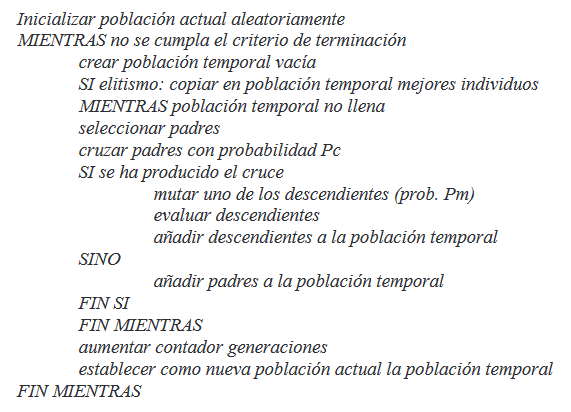
\includegraphics[width=.8\textwidth]{images/pseudocodigo.png}
    \caption{Funcionamiento algoritmo genético}
    \label{f\begin{figure}[h]
    \centering
    \includegraphics[width=.5\textwidth]{images/s\begin{figure}[h]
    \begin{figure}[h]
    \centering
    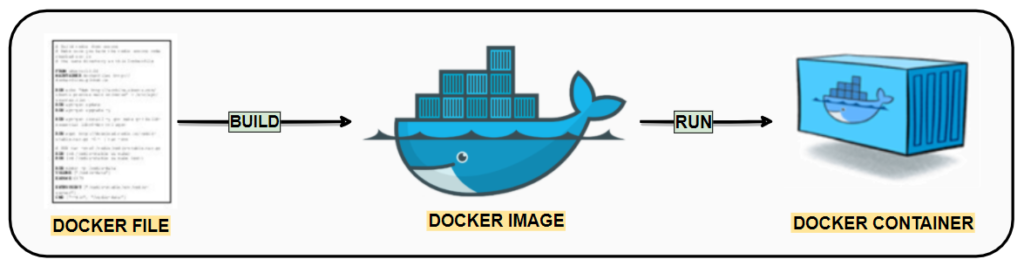
\includegraphics[width=.75\textwidth]{images/Docker2.png}
    \caption{Metodología Dockerfile}
    \label{fig:dockerfile_metodologia}
\end{figure>ring
    
\includegraphics[width=.5\textwidth]{images/logodocker.jpg}
    \caption{Logo de Docker}
    \label{fig:docker_logo}
\end{figure}ng}
    \caption{Logo de SLURM}
    \label{fig:slurm_logo}
\end{figure>udocodigo_algoritmo_genetico}
\end{figure>

El funcionamiento genérico de un algoritmo genético puede apreciarse
en el pseudocódigo, reflejado en la figura \ref{fig:pseudocodigo_algoritmo_genetico}al-Una-neurona-artificial-es-una-unidad-de.png}
    \caption{Comparacación red neuronal biológica(izquierda) y una artificial(derecha)}
    \label{fig:neurona_biologica_artificial}
\end{figure}
La inteligencia artificial (IA), en el contexto de las ciencias de la computación, es una disciplina y un conjunto de capacidades cognoscitivas e intelectuales expresadas por sistemas informáticos o combinaciones de algoritmos cuyo propósito es la creación de máquinas que imiten la inteligencia humana para realizar tareas, y que pueden mejorar conforme recopilen información\cite{espanola2014diccionario}. Se hizo presente poco después de la Segunda Guerra Mundial con el desarrollo de la "prueba de Turing", mientras que la locución fue acuñada en 1956 por el informático John McCarthy en la Conferencia de Dartmouth.

En la actualidad, la inteligencia artificial abarca una gran variedad de subcampos. Éstos van desde áreas de propósito general, aprendizaje y percepción, a otras más específicas como el reconocimiento de voz, el juego de ajedrez, la demostración de teoremas matemáticos y el diagnóstico de enfermedades. La inteligencia artificial sintetiza y automatiza tareas que en principio son intelectuales y, por lo tanto, es potencialmente relevante para cualquier ámbito de actividades intelectuales humanas. En este sentido, es un campo genuinamente universal.

La arquitectura de las inteligencias artificiales y los procesos por los cuales aprenden, se mejoran y se implementan en algún área de interés varía según el enfoque de utilidad que se les quiera dar, pero de manera general, estos van desde la ejecución de sencillos algoritmos hasta la interconexión de complejas redes neuronales artificiales que intentan replicar los circuitos neuronales del cerebro humano y que aprenden mediante diferentes modelos de aprendizaje tales como:  
\begin{itemize}
\item aprendizaje automático 
\item aprendizaje por refuerzo 
\item aprendizaje profundo 
\item aprendizaje supervisado\cite{rodriguez2017machine}.
\end{itemize}

En cuanto a su clasificación, tradicionalmente se divide a la inteligencia artificial en inteligencia artificial débil, la cual es la única que existe en la actualidad y que se ocupa de realizar tareas específicas, e inteligencia artificial fuerte, que sería una IA que excediese las capacidades humanas. Algunos expertos creen que si alguna vez se alcanza este nivel, se podría dar lugar a la aparición de una singularidad tecnológica, es decir, una entidad tecnológica superior que se mejoraría a sí misma constantemente, volviéndose incontrolable para los humanos, dando pie a teorías como el basilisco de Roko.\cite{basilico}


Stuart J. Russell y Peter Norvig diferencian varios tipos de inteligencia artificial:
\begin{itemize}
\item Los sistemas que piensan como humanos: Estos sistemas tratan de emular el pensamiento humano; por ejemplo, las redes neuronales artificiales. La automatización de actividades que vinculamos con procesos de pensamiento humano, actividades como la toma de decisiones, resolución de problemas y aprendizaje.\cite{bellman1978artificial}
\item Los sistemas que actúan como humanos: Estos sistemas tratan de actuar como humanos; es decir, imitan el comportamiento humano; por ejemplo, la robótica (El estudio de cómo lograr que los computadores realicen tareas que, por el momento, los humanos hacen mejor).\cite{winston1992artificial}
\item Los sistemas que piensan racionalmente: Es decir, con lógica (idealmente), tratan de imitar el pensamiento racional del ser humano; por ejemplo, los sistemas expertos, (el estudio de los cálculos que hacen posible percibir, razonar y actuar).\cite{winston1992artificial}
\item Los sistemas que actúan racionalmente: Tratan de emular de forma racional el comportamiento humano; por ejemplo, los agentes inteligentes, que está relacionado con conductas inteligentes en artefactos.\cite{nilsson1998artificial}
\end{itemize}


\subsection{Tipos de aprendizaje}
En cuanto a la naturaleza del aprendizaje, la IA puede subdividirse en dos campos conceptualmente distintos:
\begin{itemize}
\item El aprendizaje automático (Machine learning), que se enfoca en desarrollar algoritmos de regresión, árboles de decisión y modelos que puedan aprender de datos existentes y realizar predicciones o decisiones basadas en esos datos. En el aprendizaje automático, se utilizan técnicas de estadística matemática para encontrar patrones y relaciones en los datos y, a partir de ellos, desarrollar modelos que puedan hacer predicciones sobre nuevos datos.
\item El aprendizaje profundo (Deep learning), que se centra en la creación de redes neuronales artificiales capaces de aprender y realizar tareas de manera similar a como lo hacen los seres humanos. En el aprendizaje profundo, se utilizan capas de neuronas artificiales para procesar los datos de entrada y aprender a través de un proceso iterativo de ajuste de los pesos de las conexiones entre neuronas. Este tipo de aprendizaje es capaz de procesar y analizar grandes cantidades de datos de manera más eficiente y precisa que el primero, especialmente cuando se trata de datos no estructurados, como imágenes, texto y audio. Además, tiene la capacidad de identificar patrones y características más complejas en los datos, lo que puede llevar a mejores resultados en aplicaciones como el reconocimiento de voz, la visión por computadora y el procesamiento del lenguaje natural.
\end{itemize}


La inteligencia artificial deriva en una serie de modelos o ramas que se pueden emplear en diferentes ámbitos de la vida de las personas, así como en el mundo profesional para automatizar procesos que, realizados de manera tradicional, pueden resultar poco productivos, ineficientes, lentos o costosos.

Cada subcampo de la inteligencia artificial se encuentra en constante cambio y actualización. Por tanto, se prevé que aparezcan muchos más y que con el tiempo otros vayan quedando “obsoletos”, dejen de utilizarse, o saquen versiones mejoradas sin eliminar ese tipo de IA (como ocurre, por ejemplo, con el Deep Learning y el Machine Learning).

Se aborda dos conceptos englobados dentro de la inteligencia artificial que conforman las técnicas utilizadas en este proyecto. Esas dos técnicas son las llamadas redes neuronales artificiales y los algoritmos genéticos.

\newpage

\section{Redes neuronales artificiales}
Las redes neuronales artificiales (también conocidas como sistemas conexionistas) son un modelo computacional evolucionado a partir de diversas aportaciones científicas que están registradas en la historia.  
Consiste en un conjunto de unidades, llamadas neuronas artificiales, conectadas entre sí para transmitirse señales. La información de entrada atraviesa la red neuronal (donde se somete a diversas operaciones) produciendo unos valores de salida.
Cada neurona está conectada con otras a través de unos enlaces. En estos enlaces el valor de salida de la neurona anterior es multiplicado por un valor de peso. Estos pesos en los enlaces pueden incrementar o inhibir el estado de activación de las neuronas adyacentes. Del mismo modo, a la salida de la neurona, puede existir una función limitadora o umbral, que modifica el valor resultado o impone un límite que no se debe sobrepasar antes de propagarse a otra neurona. Esta función se conoce como función de activación.

Estos sistemas aprenden y se forman a sí mismos, en lugar de ser programados de forma explícita, y sobresalen en áreas donde la detección de soluciones o características es difícil de expresar con la programación convencional. Para realizar este aprendizaje automático, normalmente, se intenta minimizar una función de pérdida que evalúa la red en su total. Los valores de los pesos de las neuronas se van actualizando buscando reducir el valor de la función de pérdida. Este proceso se realiza mediante la propagación hacia atrás.

Los sistemas descritos son una representación basados en la manera que las neuronas actúan en todo nuestro sistema nervioso. El cerebro humano está compuesto por una gran cantidad de neuronas.
Básicamente las neuronas están formadas por: 
\begin{itemize}
    \item Un cuerpo central o Núcleo
    \item Un mecanismo de conexión con otras neuronas (sinapsis): Axón y dendritas
\end{itemize}

Los estímulos recibidos en el cerebro son transmitidos entre las neuronas mediante las conexiones sinápticas. Cuando una neurona es estimulada libera una pequeña cantidad de un componente químico (neurotransmisor). Este viaja a través del axón hasta llegar a las dendritas de otras neuronas en las cuales el proceso se repite. Este proceso sirve para incrementar o disminuir la relación entre las neuronas involucradas en él. Así, ante un determinado estímulo ciertas neuronas se activan y otras se inhiben.

Mediante un proceso de aprendizaje se logran establecer los niveles correctos de activación inhibición de las neuronas. Cuando este proceso se completa entonces ante determinados estímulos sabemos cómo responder y “aprendemos”. El “conocimiento” adquirido está entonces en los niveles de relación entre las neuronas logrados durante el proceso de aprendizaje.  El cerebro es “entrenado” por repetición de estímulos.


La misma está constituida por neuronas interconectadas y arregladas en tres capas (esto último puede variar). Los datos ingresan por medio de la “capa de entrada”, pasan a través de la “capa oculta” y salen por la “capa de salida”. Cabe mencionar que la capa oculta puede estar constituida por varias capas. Antes de comenzar el estudio sobre las redes neuronales, se debe aprender algo sobre las neuronas y de cómo ellas son utilizadas por una red neuronal. 

\begin{figure}[h]
    \centering
    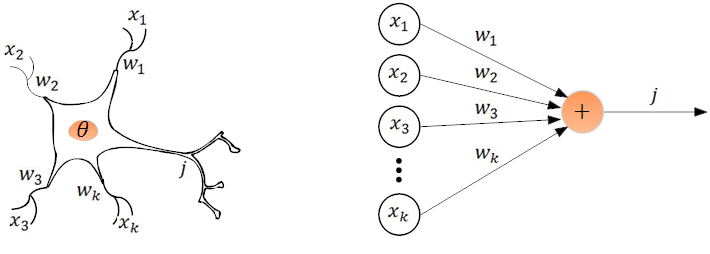
\includegraphics[width=.8\textwidth]{images/Figura-7-Neurona-biologica-versus-artificial-Una-neurona-artificial-es-una-unidad-de.png}
    \caption{Comparacación red neuronal biológica(izquierda) y una artificial(derecha)}
    \label{fig:img14}
\end{figure}

Se pueden observar las similitudes entre ambas (tienen entradas, utilizan pesos y generan salidas). 

Mientras una neurona es muy pequeña en sí misma, cuando se combinan cientos,
miles o millones de ellas pueden resolver problemas muy complejos
El objetivo de la red neuronal es resolver los problemas de la misma manera que el cerebro humano, aunque las redes neuronales son más abstractas. Las redes neuronales actuales suelen contener desde unos miles a unos pocos millones de unidades neuronales.

\subsection{Definiciones de una red neuronal}

Existen numerosas formas de definir a las redes neuronales; desde las
definiciones cortas y genéricas hasta las que intentan explicar más detalladamente qué son las redes neuronales. Por ejemplo:
\begin{itemize}
\item Una nueva forma de computación, inspirada en modelos biológicos.
\item Un modelo matemático compuesto por un gran número de elementos
  	procesales organizados en niveles.
\item Un sistema de computación compuesto por un gran número de elementos
simples, elementos de procesos muy interconectados, los cuales procesan información por medio de su estado dinámico como respuesta a entradas externas.
\item Redes neuronales artificiales son redes interconectadas masivamente en
paralelo de elementos simples (usualmente adaptativos) y con organización jerárquica, las cuales intentan interactuar con los objetos del mundo real del mismo modo que lo hace el sistema nervioso biológico.\cite{matich2001redes}
\end{itemize}

\subsection{Ventajas redes neuronales}
Debido a su constitución y a sus fundamentos, las redes neuronales artificiales presentan un gran número de características semejantes a las del cerebro. Por ejemplo, son capaces de aprender de la experiencia, de generalizar de casos anteriores a nuevos casos, de abstraer características esenciales a partir de entradas que representan información irrelevante, etc. Esto hace que ofrezcan numerosas ventajas y que este tipo de tecnología se esté aplicando en múltiples áreas. Entre las ventajas se incluyen:
\begin{itemize}
\item Aprendizaje Adaptativo. Capacidad de aprender a realizar tareas basadas en un entrenamiento o en una experiencia inicial.
\item Auto organización. Una red neuronal puede crear su propia organización o
representación de la información que recibe mediante una etapa de aprendizaje.
\item Tolerancia a fallos. La destrucción parcial de una red conduce a una
degradación de su estructura; sin embargo, algunas capacidades de la red se pueden retener, incluso sufriendo un gran daño.
\item Operación en tiempo real. Los cómputos neuronales pueden ser realizados en paralelo; para esto se diseñan y fabrican máquinas con hardware especial para obtener esta capacidad.
\item Fácil inserción dentro de la tecnología existente. Se pueden obtener chips especializados para redes neuronales que mejoran su capacidad en ciertas tareas. Ello facilitará la integración modular en los sistemas existentes.
\end{itemize}


\subsection{Fases de aprendizaje y prueba}

Existen dos fases en toda aplicación de las redes neuronales: la fase de aprendizaje o entrenamiento y la fase de prueba:
\begin{itemize}
\item Fase de Aprendizaje: una característica de las redes neuronales es su capacidad de aprender. Aprenden por la actualización o cambio de los pesos sinápticos que caracterizan a las conexiones. Los pesos son adaptados de acuerdo a la información extraída de los patrones de entrenamiento nuevos que se van presentando. Normalmente, los pesos óptimos se obtienen optimizando (minimizando o maximizando) alguna “función de energía”. Por ejemplo, un criterio popular en el entrenamiento supervisado es minimizar el least-square-error (error cuadrático medio) entre el valor deseado y el valor de salida de la red.
\item Fase de Prueba: Una vez calculados los pesos de la red, las neuronas de la última capa se comparan con la salida deseada para determinar la validez del diseño.
\end{itemize}

\subsection{Tipos de aprendizaje}
Hay dos grandes paradigmas de aprendizaje, cada uno correspondiente a una tarea de aprendizaje abstracto en particular. Estos son el aprendizaje supervisado y el aprendizaje no supervisado:
\begin{itemize}
    \item Supervisado: El aprendizaje supervisado se caracteriza porque el proceso de aprendizaje se realiza mediante un entrenamiento controlado por un agente externo (supervisor, maestro) que determina la respuesta que debería generar la red a partir de una entrada determinada. El supervisor controla la salida de la red y en caso de que ésta no coincida con la deseada, se procederá a modificar los pesos de las conexiones, con el fin de conseguir que la salida obtenida se aproxime a la deseada.
    \item No Supervisado: Las redes con aprendizaje no supervisado (también conocido como auto supervisado) no requieren influencia externa para ajustar los pesos de las conexiones entre sus neuronas. La red no recibe ninguna información por parte del entorno que le indique si la salida generada en respuesta a una determinada entrada es o no correcta.
\end{itemize}


\subsection{Función de entrada (input function)}
La neurona trata a muchos valores de entrada como si fueran uno solo; esto
recibe el nombre de entrada global. Por lo tanto, ahora nos enfrentamos al problema de cómo se pueden combinar estas simples entradas.
Los valores de entrada se multiplican por los pesos anteriormente ingresados a la neurona. Por consiguiente, los pesos que generalmente no están restringidos cambian la medida de influencia que tienen los valores de entrada. Es decir, que permiten que un gran valor de entrada tenga solamente una pequeña influencia, si estos son lo suficientemente pequeños.


\subsection{Función de activación (activation function)}
Una neurona biológica puede estar activa (excitada) o inactiva (no excitada); es decir, que tiene un “estado de activación”. Las neuronas artificiales también tienen diferentes estados de activación; algunas de ellas solamente dos, al igual que las biológicas, pero otras pueden tomar cualquier valor dentro de un conjunto determinado.
La función activación calcula el estado de actividad de una neurona; transformando la entrada global en un valor (estado) de activación, cuyo rango normalmente va de (0 a 1) o de (–1 a 1). Esto es así, porque una neurona puede estar totalmente inactiva (0 o –1) o activa (1).

\subsection{Función de salida}
El último componente que una neurona necesita es la función de salida. El valor resultante de esta función es la salida de la neurona. La función de
salida determina que valor se transfiere a las neuronas vinculadas. Si la función de activación está por debajo de un umbral determinado, ninguna salida se pasa a la neurona subsiguiente. Normalmente, no cualquier valor es permitido como una entrada para una neurona, por lo tanto, los valores de salida están comprendidos en el rango [0, 1] o [-1, 1]. También pueden ser binarios {0, 1} o {-1, 1}

\newpage
\subsection{Niveles o capas de una red neuronal}
La distribución de neuronas dentro de la red se realiza formando niveles o
capas, con un número determinado de dichas neuronas en cada una de ellas. A partir de su situación dentro de la red, se pueden distinguir tres tipos de capas:
\begin{itemize}
\item De entrada: es la capa que recibe directamente la información proveniente de las fuentes externas de la red.
\item Ocultas: son internas a la red y no tienen contacto directo con el entorno exterior. El número de niveles ocultos puede estar entre cero y un número elevado. Las neuronas de las capas ocultas pueden estar interconectadas de distintas maneras, lo que determina, junto con su número, las distintas topologías de redes neuronales.
\item De salidas: transfieren información de la red hacia el exterior. 
\end{itemize}

\newpage
\section{Algoritmos genéticos}

En los años 1970, de la mano de John Henry Holland, surgió una de las líneas más prometedoras de la inteligencia artificial, la de los algoritmos genéticos \cite{holland1992adaptation}\cite{goldberg1989algorithmsinsearch}. Son llamados así porque se inspiran en la evolución biológica y su base genético-molecular.

En la naturaleza, los procesos evolutivos ocurren cuando se satisfacen las siguientes condiciones: 
\begin{itemize}
\item Una entidad o individuo tiene la habilidad de reproducirse. 
\item Hay una población de tales individuos que son capaces de reproducirse 
\item Existe alguna variedad, diferencia, entre los individuos que se reproducen 
\item Algunas diferencias en la habilidad para sobrevivir en el entorno están asociadas con esa variedad
\end{itemize}
Los mecanismos que conducen esta evolución no son totalmente conocidos, pero sí algunas de sus características, que son ampliamente aceptadas. La evolución es un proceso que opera sobre los cromosomas más que sobre las estructuras de la vida que están codificadas en ellos.

La selección natural es el enlace entre los cromosomas y la actuación de sus estructuras decodificadas. El proceso de reproducción es el punto en el cual la evolución toma parte, actúa. La evolución biológica no tiene memoria \cite{darwin1859}.

Los algoritmos genéticos son métodos adaptativos, generalmente usados
en problemas de búsqueda y optimización de parámetros, basados en la reproducción sexual y en el principio de supervivencia del más apto. \cite{fogel2000evolutionary} \cite{fogel2006evolutionary}.

Más formalmente, y siguiendo la definición dada por David E. Goldberg, “los algoritmos genéticos son algoritmos de búsqueda basados en la mecánica de selección natural y de la genética natural. Combinan la supervivencia del más apto entre estructuras de secuencias con un intercambio de información estructurado, aunque aleatorizado, para constituir así un algoritmo de búsqueda que tenga algo de las genialidades de las búsquedas humanas” \cite{goldberg1989artificial}.


Para alcanzar la solución a un problema se parte de un conjunto inicial de individuos, llamado población, generado de manera aleatoria. Cada uno de estos individuos representan una posible solución al problema. Estos individuos evolucionarán tomando como base los esquemas propuestos por Darwin sobre la selección natural, y se adaptarán en mayor medida tras el paso de cada generación a la solución requerida \cite{darwin2007}.

Estos algoritmos hacen evolucionar una población de individuos sometiéndola a acciones aleatorias, semejantes a las que actúan en la evolución biológica (mutaciones y recombinaciones genéticas), así como también a una selección. De acuerdo con algún criterio, se decide cuáles son los individuos más adaptados, que sobreviven, y cuáles son los menos aptos, que son descartados.

Los algoritmos genéticos trabajan sobre una población de individuos. Cada uno de ellos representa una posible solución al problema que se desea resolver. Todo individuo tiene asociado un ajuste de acuerdo a la bondad con respecto al problema de la solución que representa (en la naturaleza el equivalente sería una medida de la eficiencia del individuo en la lucha por los recursos). Una generación se obtiene a partir de la anterior por medio de los operadores de reproducción\cite{algGen2014}. Existen 2 tipos:
\begin{itemize}
\item Cruce. Se trata de una reproducción de tipo sexual. Se genera una descendencia a partir del mismo número de individuos (generalmente 2) de la generación anterior. Existen varios tipos que se detallarán en un punto posterior.
\item Copia. Se trata de una reproducción de tipo asexual. Un determinado número de individuos pasa sin sufrir ninguna variación directamente a la siguiente generación.
\end{itemize}


\begin{figure}[h]
    \centering
    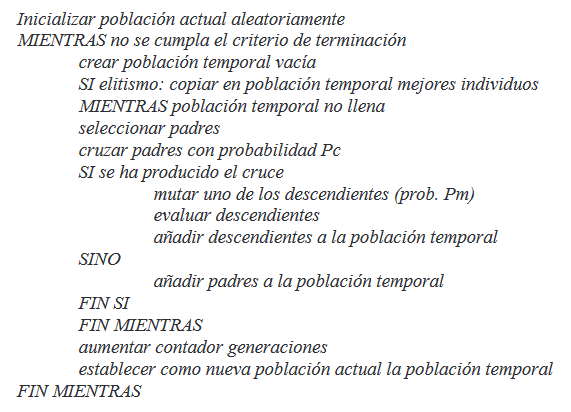
\includegraphics[width=.8\textwidth]{images/pseudocodigo.png}
    \caption{Funcionamiento algoritmo genético}
    \label{fig:img14}
\end{figure}

El funcionamiento genérico de un algoritmo genético puede apreciarse
en el pseudocódigo, reflejado en la figura \ref{fig:img14}

Si desea optarse por una estrategia elitista, los mejores individuos de cada
generación se copian siempre en la población temporal, para evitar su pérdida.
A continuación, comienza a generarse la nueva población en base a la aplicación de los operadores genéticos de cruce y/o copia. Una vez generados los nuevos individuos se realiza la mutación en función a una probabilidad estipulada. 

Se sale de este proceso cuando se alcanza alguno de los criterios de parada fijados. Los más usuales suelen ser:
\begin{itemize}
\item Los mejores individuos de la población representan soluciones suficientemente buenas para el problema que se desea resolver.
\item La población ha convergido. Un gen ha convergido cuando el 95\% de la población tiene el mismo valor para él, en el caso de trabajar con codificaciones binarias, o valores dentro de un rango especificado en el caso de trabajar con otro tipo de codificaciones. Una vez que todos los genes alcanzan la convergencia se dice que la población ha convergido. Cuando esto ocurre la media de bondad de la población se aproxima a la bondad del mejor individuo.
\item Se ha alcanzado el número de generaciones máximo especificado.
\end{itemize}

Para el paso de una generación a la siguiente se aplican una serie de operadores genéticos. Los más empleados son los operadores de selección, cruce y mutación. En el caso de no trabajar con una población intermedia temporal también cobran relevancia los algoritmos de reemplazo. A continuación, se verán en mayor detalle.


\subsection {Selección} 

Los algoritmos de selección serán los encargados de escoger qué individuos van a disponer de oportunidades de reproducirse y cuáles no. Puesto que se trata de imitar lo que ocurre en la naturaleza, se ha de otorgar un mayor número de oportunidades de reproducción a los individuos más aptos. Por lo tanto, la selección de un individuo estará relacionada con su valor de ajuste. No se debe, sin embargo, eliminar por completo las opciones de reproducción de los individuos menos aptos, pues en pocas generaciones la población se volvería homogénea.


\subsubsection {Selección por ruleta}

A cada uno de los individuos de la población se le asigna una parte proporcional a su ajuste de una ruleta, de tal forma que la suma de todos los porcentajes sea la unidad. Los mejores individuos recibirán una porción de la ruleta mayor que la recibida por los peores. Generalmente, la población está ordenada en base al ajuste, por lo que las porciones más grandes se encuentran al inicio de la ruleta. Para seleccionar un individuo basta con generar un número aleatorio del intervalo [0…1] y devolver el individuo situado en esa posición de la ruleta. Esta posición se suele obtener recorriendo los individuos de la población y acumulando sus proporciones de ruleta hasta que la suma exceda el valor obtenido.

Esta selección permite que los mejores individuos sean elegidos con una mayor probabilidad, pero al mismo tiempo permite a los peores individuos ser elegidos, lo cual puede ayudar a mantener la diversidad de la población.


\subsubsection {Selección por truncamiento}

En esta selección las soluciones candidatas son ordenadas según su función de desempeño, y una proporción p (por ejemplo =1/2, 1/3, 1/4, ...) de los individuos con mejor desempeño es seleccionada y reproducida 1/p veces. Esta selección es menos
sofisticada que la mayoría de los métodos de selección.


\subsubsection{Selección basada en ranking}

En esta selección los individuos se ordenan según su medida de desempeño y luego son asignados con una segunda medida de desempeño, inversamente proporcional a su posición en el ranking (esto es, otorgando una mayor probabilidad a los mejores). Los valores de esta segunda asignación pueden ser lineales o exponenciales. Finalmente, los individuos son seleccionados proporcionalmente a esta probabilidad. 

Este método disminuye el riesgo de convergencia prematura (En los algoritmos evolutivos, el término de convergencia prematura significa que una población para un problema de optimización convergió demasiado pronto, lo que resultó en una subóptima) que se produce cuando se utiliza selección de ruleta en poblaciones con unos pocos individuos con medidas de desempeño muy superiores a las del resto.



\subsubsection{Selección por torneo}
Esta selección se efectúa mediante un torneo (comparación) entre un pequeño subconjunto de individuos elegidos al azar desde la población. Los beneficios de este tipo de selección son la velocidad de aplicación (dado que no es necesario evaluar ni comparar la totalidad de la población) y la capacidad de prevenir, en cierto grado, la convergencia prematura. La principal desventaja es la necesidad de establecer el parámetro correspondiente al tamaño del subconjunto.

\label{sec:MachineLearning}


\subsection{Cruce}

Una vez seleccionados los individuos, éstos son recombinados para producir la descendencia que se insertará en la siguiente generación. Tal y como se ha indicado anteriormente, el cruce es una estrategia de reproducción sexual. Su importancia para la transición entre generaciones es elevada puesto que las tasas de cruce con las que se suele trabajar rondan el 90\%. Los diferentes métodos de cruce podrán operar de dos formas diferentes. Si se opta por una estrategia destructiva los descendientes se insertarán en la población temporal, aunque sus padres tengan mejor ajuste (trabajando con una única población esta comparación se realizará con los individuos a reemplazar). Por el contrario, utilizando una estrategia no destructiva la descendencia pasará a la siguiente generación únicamente si supera la bondad del ajuste de los padres (o de los individuos a reemplazar). La idea principal del cruce se basa en que, si se toman dos individuos correctamente adaptados al medio y se obtiene una descendencia que comparta genes de ambos, existe la posibilidad de que los genes heredados sean precisamente los causantes de la bondad de los padres. Al compartir las características buenas de dos individuos, la descendencia, o al menos parte de ella, debería tener una bondad mayor que cada uno de los padres por separado. Si el cruce no agrupa las mejores características en uno de los hijos y la descendencia tiene un peor ajuste que los padres no significa que se esté dando un paso atrás. Optando por una estrategia de cruce no destructiva garantizamos que pasen a la siguiente generación los mejores individuos. Si, aún con un ajuste peor, se opta por insertar a la descendencia, y puesto que los genes de los padres continuarán en la población –aunque dispersos y posiblemente levemente modificados por la mutación–, en posteriores cruces se podrán volver a obtener estos padres, recuperando así la bondad previamente perdida.
Existen multitud de algoritmos de cruce. Sin embargo, los más empleados
son los que se detallarán a continuación:
\begin{itemize}
\item Cruce de 1 punto
\item Cruce de 2 puntos
\item Cruce uniforme
\end{itemize}


\subsubsection{Cruce en 1 punto}\label{cruce1punto}
Se selecciona un punto en el vector del primer parental. Todos los datos más allá de este punto en el vector del organismo se intercambiarán entre los dos organismos parentales. Los organismos resultantes son los hijos:


\subsubsection{Cruce en 2 punto}\label{cruce2puntos}
Se selecciona un punto en el vector del primer parental. Todos los datos más allá de este punto en el vector del organismo se intercambiarán entre los dos organismos parentales. Los organismos resultantes son los hijos:

\subsubsection{Cruce uniforme}\label{cruceuniforme}

En el esquema de recombinación uniforme, los bits del vector se comparan individualmente entre ambos padres. Los bits se intercambian con una probabilidad fijada, usualmente 0.5.

En el esquema de recombinación uniforme media, exactamente la mitad de los bits que son diferentes se intercambian. Este número se divide entre dos, y el número resultante es la cantidad de bits diferentes que tiene que ser intercambiada entre los parentales.


Otra forma de implementar esta recombinación es generando una máscara que determina que valores de cada padre van hacia cada nuevo hijo generado. Si en una de las posiciones de la máscara hay un 1, el gen situado en esa posición en uno de los descendientes se copia del primer padre. Si por el contrario hay un 0 el gen se copia del segundo padre. Para producir el segundo descendiente se intercambian los papeles de los padres, o bien se intercambia la interpretación de los unos y los ceros de la máscara de cruce.


\subsection{Mutación}
La mutación de un individuo provoca que alguno de sus genes, general-
mente uno sólo, varíe su valor de forma aleatoria. Aunque se pueden seleccionar los individuos directamente de la población actual y mutarlos antes de introducirlos en la nueva población, la mutación se suele utilizar de manera conjunta con el operador de cruce. 
Primeramente, se seleccionan dos individuos de la población para realizar el cruce. Si el cruce tiene éxito entonces uno de los descendientes, o ambos, se muta en función a cierta probabilidad . Se imita de esta manera el comportamiento que se da en la naturaleza, pues cuando se genera la descendencia siempre se produce algún tipo de error, por lo general sin mayor trascendencia, en el paso de la carga genética de padres a hijos.
El propósito de la mutación es proveer un mecanismo para escapar abruptamente de los óptimos locales, así como desplazar a los individuos hacia zonas del espacio de búsqueda que no pueden ser alcanzadas por medio de otros operadores genéticos.

Puede consistir en el cambio de un bit aleatorio, de uno a cero o de cero a uno.
Ejemplo:

\begin{figure}[h]
    \centering
    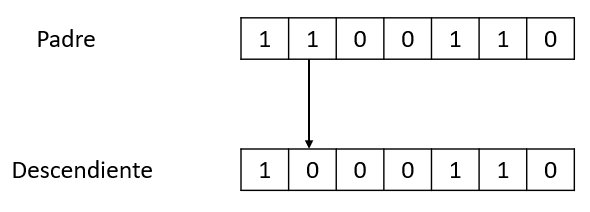
\includegraphics[width=.5\textwidth]{images/mutacion1.png}
    \caption{Ejemplo mutación simple}
    \label{fig:img0}
\end{figure}


O, por el contrario. Puede consistir en intercambiar dos posiciones.
Ejemplo:

\begin{figure}[h]
    \centering
    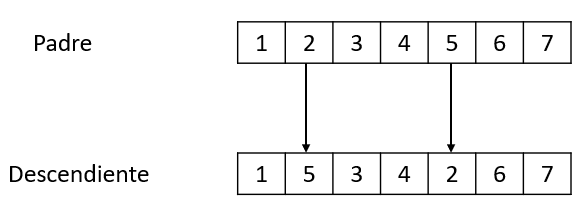
\includegraphics[width=.5\textwidth]{images/mutacion2.png}
    \caption{Ejemplo mutación de intercambio de posiciones}
    \label{fig:img1}
\end{figure}


\subsection{Elitismo}
El elitismo es un caso particular donde pasamos a la siguiente población generada en la siguiente iteración el mejor o mejores individuos de una generación en la generación siguiente. De esta manera se garantiza que el proceso de búsqueda nunca dará un paso atrás en cuanto a la calidad de la mejor solución obtenida, sino que un cambio en ésta siempre implicará una mejora. Una variación de este proceso consiste en copiar al mejor o mejores individuos de una generación en la siguiente, únicamente cuando tras el paso de una generación no se haya mejorado con los operadores de cruce o mutación la mejor solución de la generación actual.

\subsection{Reemplazo}\label{reemplazamiento}
Una vez aplicados los operadores genéticos, se seleccionan los mejores individuos para conformar la población de la generación siguiente. La presión selectiva se ve también afectada por la forma en que los cromosomas de la población son reemplazados por los nuevos descendientes. Se pueden utilizar métodos de reemplazamiento aleatorios o deterministas:

\begin{itemize}
    \item Reemplazamiento generacional: se reemplaza toda la población actual con los descendientes generados.
    \item Reemplazamiento estacionario: se tomas los padres y los descendientes generados, son comparados entre ellos y los dos mejores de estos cuatro individuos son los que se añaden a la nueva población generada.
\end{itemize}


\subsection{Evaluación}
Para el correcto funcionamiento de un algoritmo genético se debe de poseer un método que indique si los individuos de la población representan o no buenas soluciones al problema planteado. Por lo tanto, para cada tipo de problema que se desee resolver deberá derivarse un nuevo método, al igual que ocurrirá con la propia codificación de los individuos.
De esto se encarga la función de evaluación, que establece una medida numérica de la bondad de una solución. Esta medida recibe el nombre de ajuste. En la naturaleza el ajuste (o adecuación) de un individuo puede considerarse como la probabilidad de que ese individuo sobreviva hasta la edad de reproducción y se reproduzca. En el mundo de los algoritmos genéticos se empleará esta medición para controlar la aplicación de los operadores genéticos. Es decir, permitirá controlar el número de selecciones, cruces y mutaciones llevadas a cabo. La aproximación más común consiste en crear explícitamente una medida de ajuste para cada individuo de la población. A cada uno de los individuos se le asigna un valor de ajuste escalar por medio de un procedimiento de evaluación bien definido. Tal y como se ha comentado, este procedimiento de evaluación será específico del dominio del problema en el que se aplica el algoritmo genético.


\newpage

\section{Herramientas a utilizar}
\subsection{Anaconda}

\begin{figure}[h]
    \centering
    
\includegraphics[width=.5\textwidth]{images/anaconda.png}
    \caption{Logo de Anaconda}
    \label{fig:img2}
\end{figure}
Anaconda es una distribución libre y abierta de los lenguajes Python y R, utilizada en ciencia de datos, y aprendizaje automático (machine learning). Esto incluye procesamiento de grandes volúmenes de información, análisis predictivo y cómputos científicos. Está orientado a simplificar el despliegue y administración de los paquetes de software. 

Las diferentes versiones de los paquetes se administran mediante el sistema de gestión de paquetes conda, el cual lo hace bastante sencillo de instalar, correr, y actualizar software de ciencia de datos y aprendizaje automático como puede ser Scikit-team, TensorFlow y SciPy. 

La distribución Anaconda es utilizada por 6 millones de usuarios e incluye más de 250 paquetes de ciencia de datos válidos para Windows, Linux y MacOS.
Para ejecutarse, muchos paquetes científicos dependen de versiones específicas de otros paquetes. Los paquetes científicos a menudo usan múltiples versiones de muchos paquetes y utilizan múltiples entornos para separar estas diferentes versiones.

Conda es tanto un administrador de paquetes como un administrador de entorno. Esto ayuda a los usuarios a asegurarse de que cada versión de cada paquete tenga todas las dependencias que requiere y funcione correctamente.

El mundo de la inteligencia artificial y de la ciencia y análisis de datos está muy ligado a Python y esto implica, necesariamente, adaptarse a las particularidades de este mundo. Anaconda viene tanto a solucionar la entrada a los que se inicien en este apasionante mundo como a ser una herramienta imprescindible en el día a día para los científicos de datos más experimentados gestionando por nosotros entornos, librerías o paquetes etc. Desde luego, es una solución muy recomendable para el día a día del análisis de datos.
\newpage

\subsection{Simple Linux Utility for Resource Management(SLURM)}

\begin{figure}[h]
    \centering
    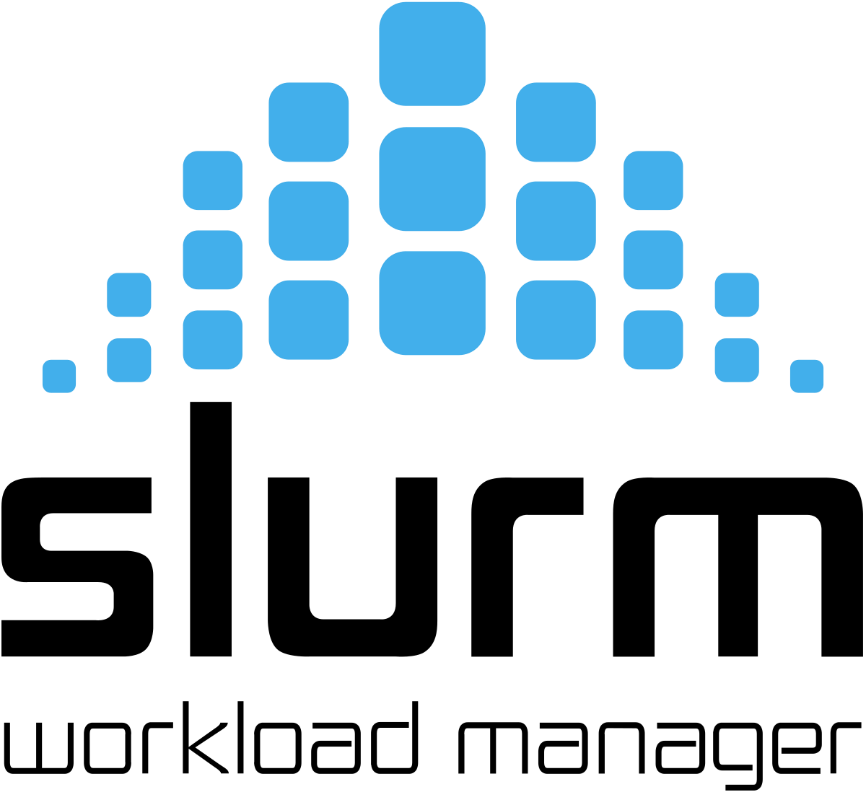
\includegraphics[width=.5\textwidth]{images/slurm.png}
    \caption{Logo de SLURM}
    \label{fig:img3}
\end{figure}

Slurm es un sistema de programación de trabajos y administración de clústeres de código abierto, tolerante a fallas y altamente escalable para clústeres de Linux grandes y pequeños. Slurm no requiere modificaciones del kernel para su funcionamiento y es relativamente autónomo. Como administrador de cargas de trabajo de clúster, Slurm tiene tres funciones clave. Primero, asigna acceso exclusivo y/o no exclusivo a los recursos (nodos de computación) a los usuarios durante un período de tiempo para que puedan realizar su trabajo. En segundo lugar, proporciona un marco para iniciar, ejecutar y monitorear el trabajo (normalmente un trabajo paralelo) en el conjunto de nodos asignados. Finalmente, arbitra la contienda por los recursos gestionando una cola de trabajos pendientes. Se pueden utilizar complementos opcionales para contabilidad, reserva avanzada, programación grupal (tiempo compartido para trabajos paralelos), programación de reabastecimiento, selección de recursos optimizada por topología, límites de recursos por usuario o cuenta bancaria y sofisticados algoritmos de priorización de trabajos multifactorial.
En SLURM, debemos de diferenciar dos tipos de roles (que se corresponden con los distintos tipos de usuarios del sistema), que son los “usuarios” y los “administradores”. Ambos interactúan con SLURM mediante un conjunto de comando simples, pero sus propósitos son totalmente contrapuestos:

\begin{itemize}
\item Usuarios: Envían trabajos para que se ejecuten, y esperan a que finalice lo más rápido posible y de manera correcta, sin importarles si el trabajo se ha realizado en uno, dos o tres nodos de cómputo.
\item Administradores: Debe encontrar la manera de ejecutar trabajos paralelos en nodos paralelos, y lo que es más importante, deben hacer como si el trabajo se ejecutará en un solo nodo. Las tareas de un administrador son:
\begin{itemize}
\item Asignar recursos de un nodo de cómputo: Procesadores, memoria, espacio en disco…etc.
\item Lanzar y administrar trabajos.
\end{itemize}
\end{itemize}

Una vez visto cómo se ejecuta un trabajo, es interesante ver los estados por los que puede pasar cada uno de ellos.
\begin{enumerate}
\item Pending: Trabajo en cola.
\item Running: Recursos asignados y trabajo en ejecución.
\item Suspended: Recursos asignados y trabajo suspendido.
\item Completing:
\begin{itemize}
\item Cancelled: Trabajo cancelado por el usuario.
\item Completed: Trabajo finalizado correctamente.
\item Failed: Ejecución finalizada incorrectamente.
\item NodeFail: Terminado por fallo en el nodo.
\item TimeOut: Terminado por alcanzar el TimeOut.
\end{itemize}
\end{enumerate}


\begin{table}[h] %usamos h para poner debajo del titulo
    \centering
    \begin{adjustbox}{max width=1.3\textwidth,center}
    \scalebox{0.5}{
    \begin{tabular}{|c|l|} %l = left r = rigth c = center
    \hline
    Comando  &  \multicolumn{1}{|c|}{Descripción}    \\
    \hline
    srun & Envía un trabajo para su ejecución  \\
    \hline
    scancel & Finaliza trabajos que se encuentren en ejecución o pendientes \\
    \hline
    sinfo & Muestra información sobre el estado de los nodos de cómputo \\
    \hline
    squeue & Informa sobre el estado de los trabajos en ejecución en orden de prioridad \\ & y luego de los trabajos pendientes también en orden de prioridad \\
    \hline
    sacct & Da información acerca de trabajos completados o que se encuentren activos \\
    \hline
    smap & Muestra información del estado de los trabajos, particiones y nodos de cómputo, \\ & pero muestra la información gráficamente para reflejar la topología de la red \\
    \hline
    sview & Interfaz gráfica para obtener información acerca del estado de los trabajos, \\ & particiones y nodos de cómputo  \\
    \hline
    salloc & Asigna recursos para un trabajo en tiempo real \\
    \hline
    sattach & Añade una entrada o salida estándar a un trabajo \\
    \hline
    sbatch & Envía un script para su posterior ejecución \\
    \hline
    sbcast & Se utiliza para mandar un archivo a los nodos de cómputo asignados a un trabajo \\
    \hline
    sacctmgr & Herramienta para gestionar la base de datos  \\
    \hline
    scontrol & Herramienta administrativa que se utiliza para ver o modificar el estado de SLURM.\\ & Muchos comandos control sólo podrán ser ejecutados como root strigger. \\ & Nos permite ver, obtener o establecer eventos de activación \\
    \hline
    \end{tabular}
    }
    \end{adjustbox}
    \caption{Comandos SLURM}
    \label{tab:tablaslurm}
\end{table}

\newpage
\subsection{Docker}\label{docker}

\begin{figure}[h]
    \centering
    
\includegraphics[width=.5\textwidth]{images/logodocker.jpg}
    \caption{Logo de Docker}
    \label{fig:img3}
\end{figure}

Docker es una plataforma de software que le permite crear, probar e implementar aplicaciones rápidamente. Docker empaqueta software en unidades estandarizadas llamadas contenedores que incluyen todo lo necesario para que el software se ejecute, incluidas bibliotecas, herramientas de sistema, código y tiempo de ejecución. Con Docker, puede implementar y ajustar la escala de aplicaciones rápidamente en cualquier entorno con la certeza de saber que su código se ejecutará.

Docker le proporciona una manera estándar de ejecutar su código. Docker es un sistema operativo para contenedores. De manera similar a cómo una máquina virtual virtualiza (elimina la necesidad de administrar directamente) el hardware del servidor, los contenedores virtualizan el sistema operativo de un servidor. Docker se instala en cada servidor y proporciona comandos sencillos que puede utilizar para crear, iniciar o detener contenedores.

La tecnología utilizada se engloba en lo que se conoce como Dockerfile.
Un Dockerfile es un archivo o documento de texto simple que incluye una serie de instrucciones que se necesitan ejecutar de manera consecutiva para cumplir con los procesos necesarios para la creación de una nueva imagen.

A este conjunto de instrucciones se le conoce como línea de comandos y serán los encargados de indicar los pasos a seguir para el ensamblaje de una imagen en Docker, es decir, los elementos necesarios para el desarrollo de un contenedor en Docker.

De manera que las imágenes en docker file se crean a partir de un comando en específico denominado docker build, que se encargará de ofrecer las herramientas para que el sistema siga las instrucciones que el usuario haya indicado en la línea de comandos.

\begin{figure}[h]
    \centering
    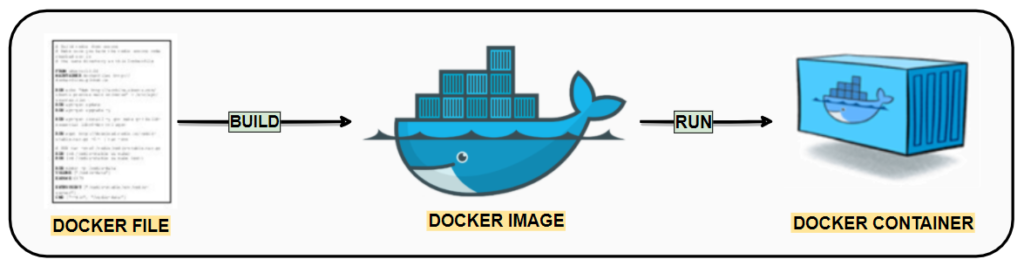
\includegraphics[width=.75\textwidth]{images/Docker2.png}
    \caption{Metodología Dockerfile}
    \label{fig:img3}
\end{figure}



\subsection{Componentes físicos}
Para que este proyecto se haya podido llevar a cabo, se ha posibilitado el uso de un servidor Supermicro 4U Dual Xeon LGA4189. Este ha sido imprescindible para todo el desarrollo de este proyecto, permitiendo la instalación y utilización de las distintas herramientas de software ya definidas en este capítulo anteriormente, así como la ejecución de los distintos procesos necesarios, gracias la alta capacidad de procesamiento. Además proporciona la posibilidad de llevar a cabo las ejecuciones necesarias de manera paralela gracias a las 4 GPUs que posee, facilitando la tarea y minimizando el tiempo utilizado para ello.


\vspace{1cm}
